\section{Einfluss eines Magneten auf Wasser - Eine Fermi-Abschätzung. }
\subsection{Methoden}
Um den Einfluss eine Magnetfeldes zu untersuchen wurde ein Laser auf eine Wasseroberfläche gerichtet. Unter dem Behälter mit dem Wasser (einer Petrischale) wurde dann ein Magnet drunter hergeschoben. Anhand der Bewegung des auf eine Wand reflektierten Lasers konnte man erkennen auf welche Art das Wasser beeinflusst wurde.
Um einschätzen zu könne wie groß der Einfluss des Magnetfeldes war wurden alle für die Rechnung relevanten Werte abgeschätzt.bei dieser Abschätzung handelte es sich um eine Fermi-Abschätzung. Das heißt man schätzt die werte grob ab und geht davon aus das die Unsicherheiten sich gegenseitig aufheben. Diese Abschätzung liefert keine genauen werte, jedoch liefert sie einen guten Hinweis  auf die Größenordnungen in der man sich bewegt.
\subsection{Ergebnisse}
Beim durchführen des Experimentes fiel auf das sich der Laserpunkt erst nach oben und dann nach unten bewegte. Dies ist darauf zurückzuführen das Wasser Diamagnetisch ist, also aus Magnetfeldern Verdrängt wird. Das führt dazu das sich eine Einbuchtung in der Oberfläche bildet die bei der Rechnung durch ein Dreieck Approximiert wurde.
Die Abschätzung der Relevanten Werte lieferte, für einen Versuchsaufbau ähnlich zu \cref{fig:aufbau} , für $x=\SI{400}{cm}, y=\SI{130}{cm}, \Delta y\SI{+- 3,5}{cm}$ und $d=\SI{1}{cm}$ (Die Bedeutungen der einzelnen Werte sind in \cref{fig:Skizze} zu sehen). Mithilfe einiger Trigonometrischer Zusammenhänge kommt man dann auf die Gleichungen:
\begin{align}
	2\beta &= \arctan \left(\frac{\Delta y + y}{x}\right)  - \arctan\left( \frac{y}{x}\right)\\ 
	\tan(\beta) &= \frac{2h}{d}
\end{align}
Setzt man diese Gleichungen ineinander ein und stellt sie nach $h$ um erhält man für einen Wert für $h$ von \SI{0,00198}{cm}.Magnetfeldes auf Wasser nur sehr klein ist. Da Wasser Diamagnetisch ist und Diamagnetismus meist nur sehr schwach auftritt entspricht die Größenordnung des erhaltenen Wertes der Erwarteten Größenordnung.
Wie schon zu beginn festgestellt wurde handelt es sich bei diesem wert nicht um einen Exakten wert sondern nur um einen Näherungswert, was auf die Art und weise zurückzuführen ist wie die Werte abgeschätzt wurden.



	\begin{figure}[h]
		
		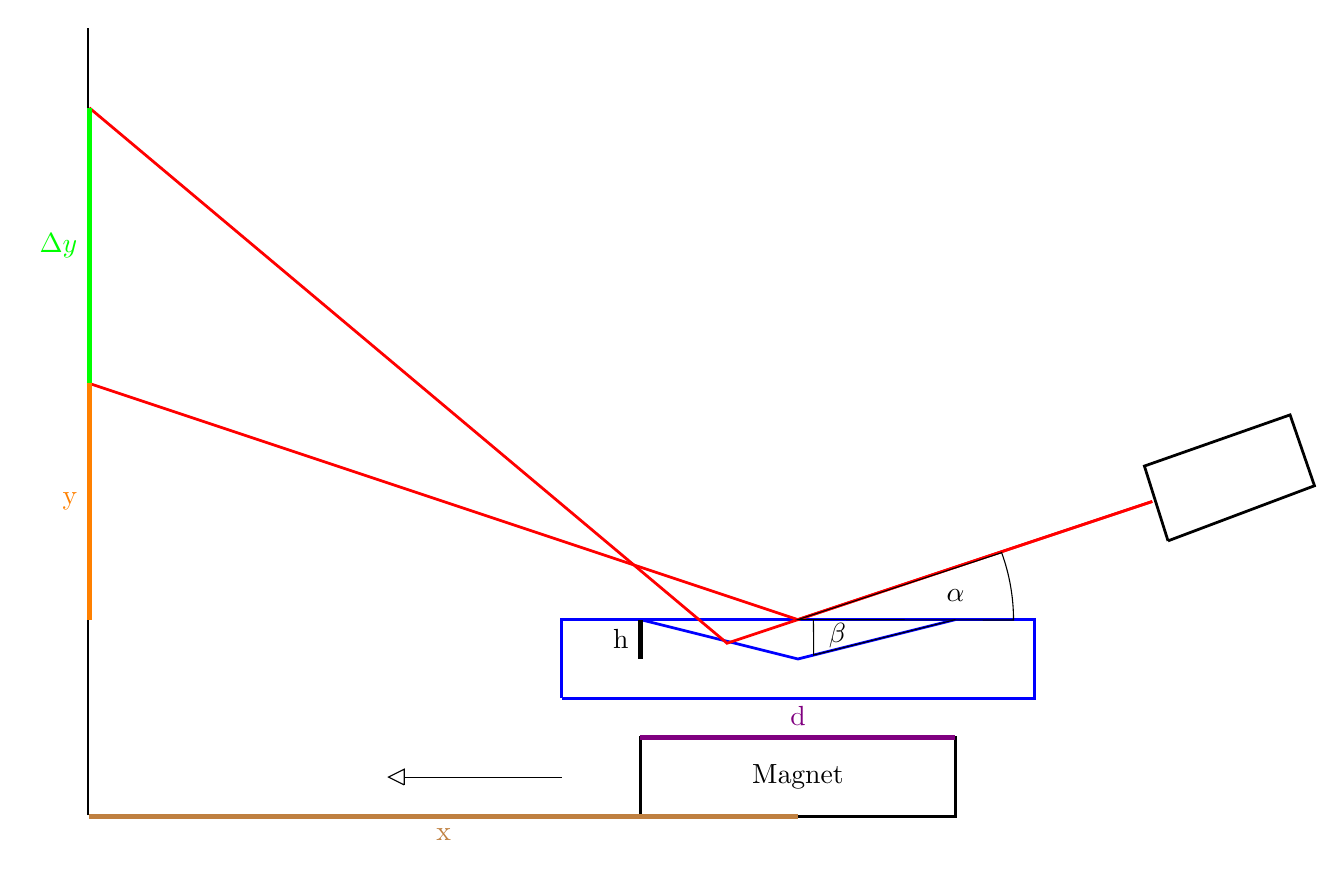
\begin{tikzpicture}[scale=1]
		\tikz 
		\draw[line width=1pt] (0,0) -- (0,10); %Wand
		\draw[line width=1pt, color=blue] (6,1.5) -- (6,2.5) -- (12,2.5) -- (12,1.5) -- (6,1.5); %Wasser
		\draw[line width=1pt, color=blue] (7,2.5) -- (9,2) -- (11,2.5); %Wasser dreieck
		\draw[line width=1pt] (7,0) -- (7,1) -- (11,1) -- (11,0) -- (7,0) node at (9,0.5){Magnet}; % Magnet
		\draw[line width=1pt] (13.7,3.5) -- (15.56,4.2) -- (15.25,5.1) -- (13.4,4.45) --(13.7,3.5) ; % Laser
		\draw [line width=1pt, color=red] (13.5,4) -- (9,2.5) -- (0,5.5) ; %lichtstrahl 1
		\draw [line width=1pt, color=red] (13.5,4) --(8.1,2.2) -- (0,9); %Lichtstrahl 2 
		\draw[black] (9,2.5) -- (12:12) arc (0:20:2.5) -- cycle node at (11,2.8) {$\alpha$};
		\draw[black] (11,2.5) -- (9.2,2.05) arc (0:0.9:29) node at (9.5,2.3) {$\beta$};
		\draw [line width=2pt, color=green] (0,5.5) -- (0,9) node[midway, left] {$\Delta y$}  ;
		\draw [line width=2pt, color= orange](0,2.5) -- (0,5.5) node[midway, left]{y};
		\draw [line width=2pt, color=violet] (7,1)--(11,1) node [midway, above] {d};
		\draw[line width=2pt, color=brown] (0,0)--(9,0) node[midway, below] {x};
		\draw[line width=2pt] (7,2) -- (7,2.5) node[midway, left]{h};
		\draw (6,0.5) -> (4,0.5);
		\draw (4,0.4) -- (4,0.6) -- (3.8,0.5)-- (4,0.4);
		\end{tikzpicture}
		\caption{Skizze des Versuchsaufbaus. Hier ist jedoch nur einer der beiden beobachteten Fälle betrachtet. Der Fall für $-\Delta y$ ist nicht explizit aufgeführt. }
		\label{fig:Skizze}
	\end{figure}
\begin{figure}[h]
	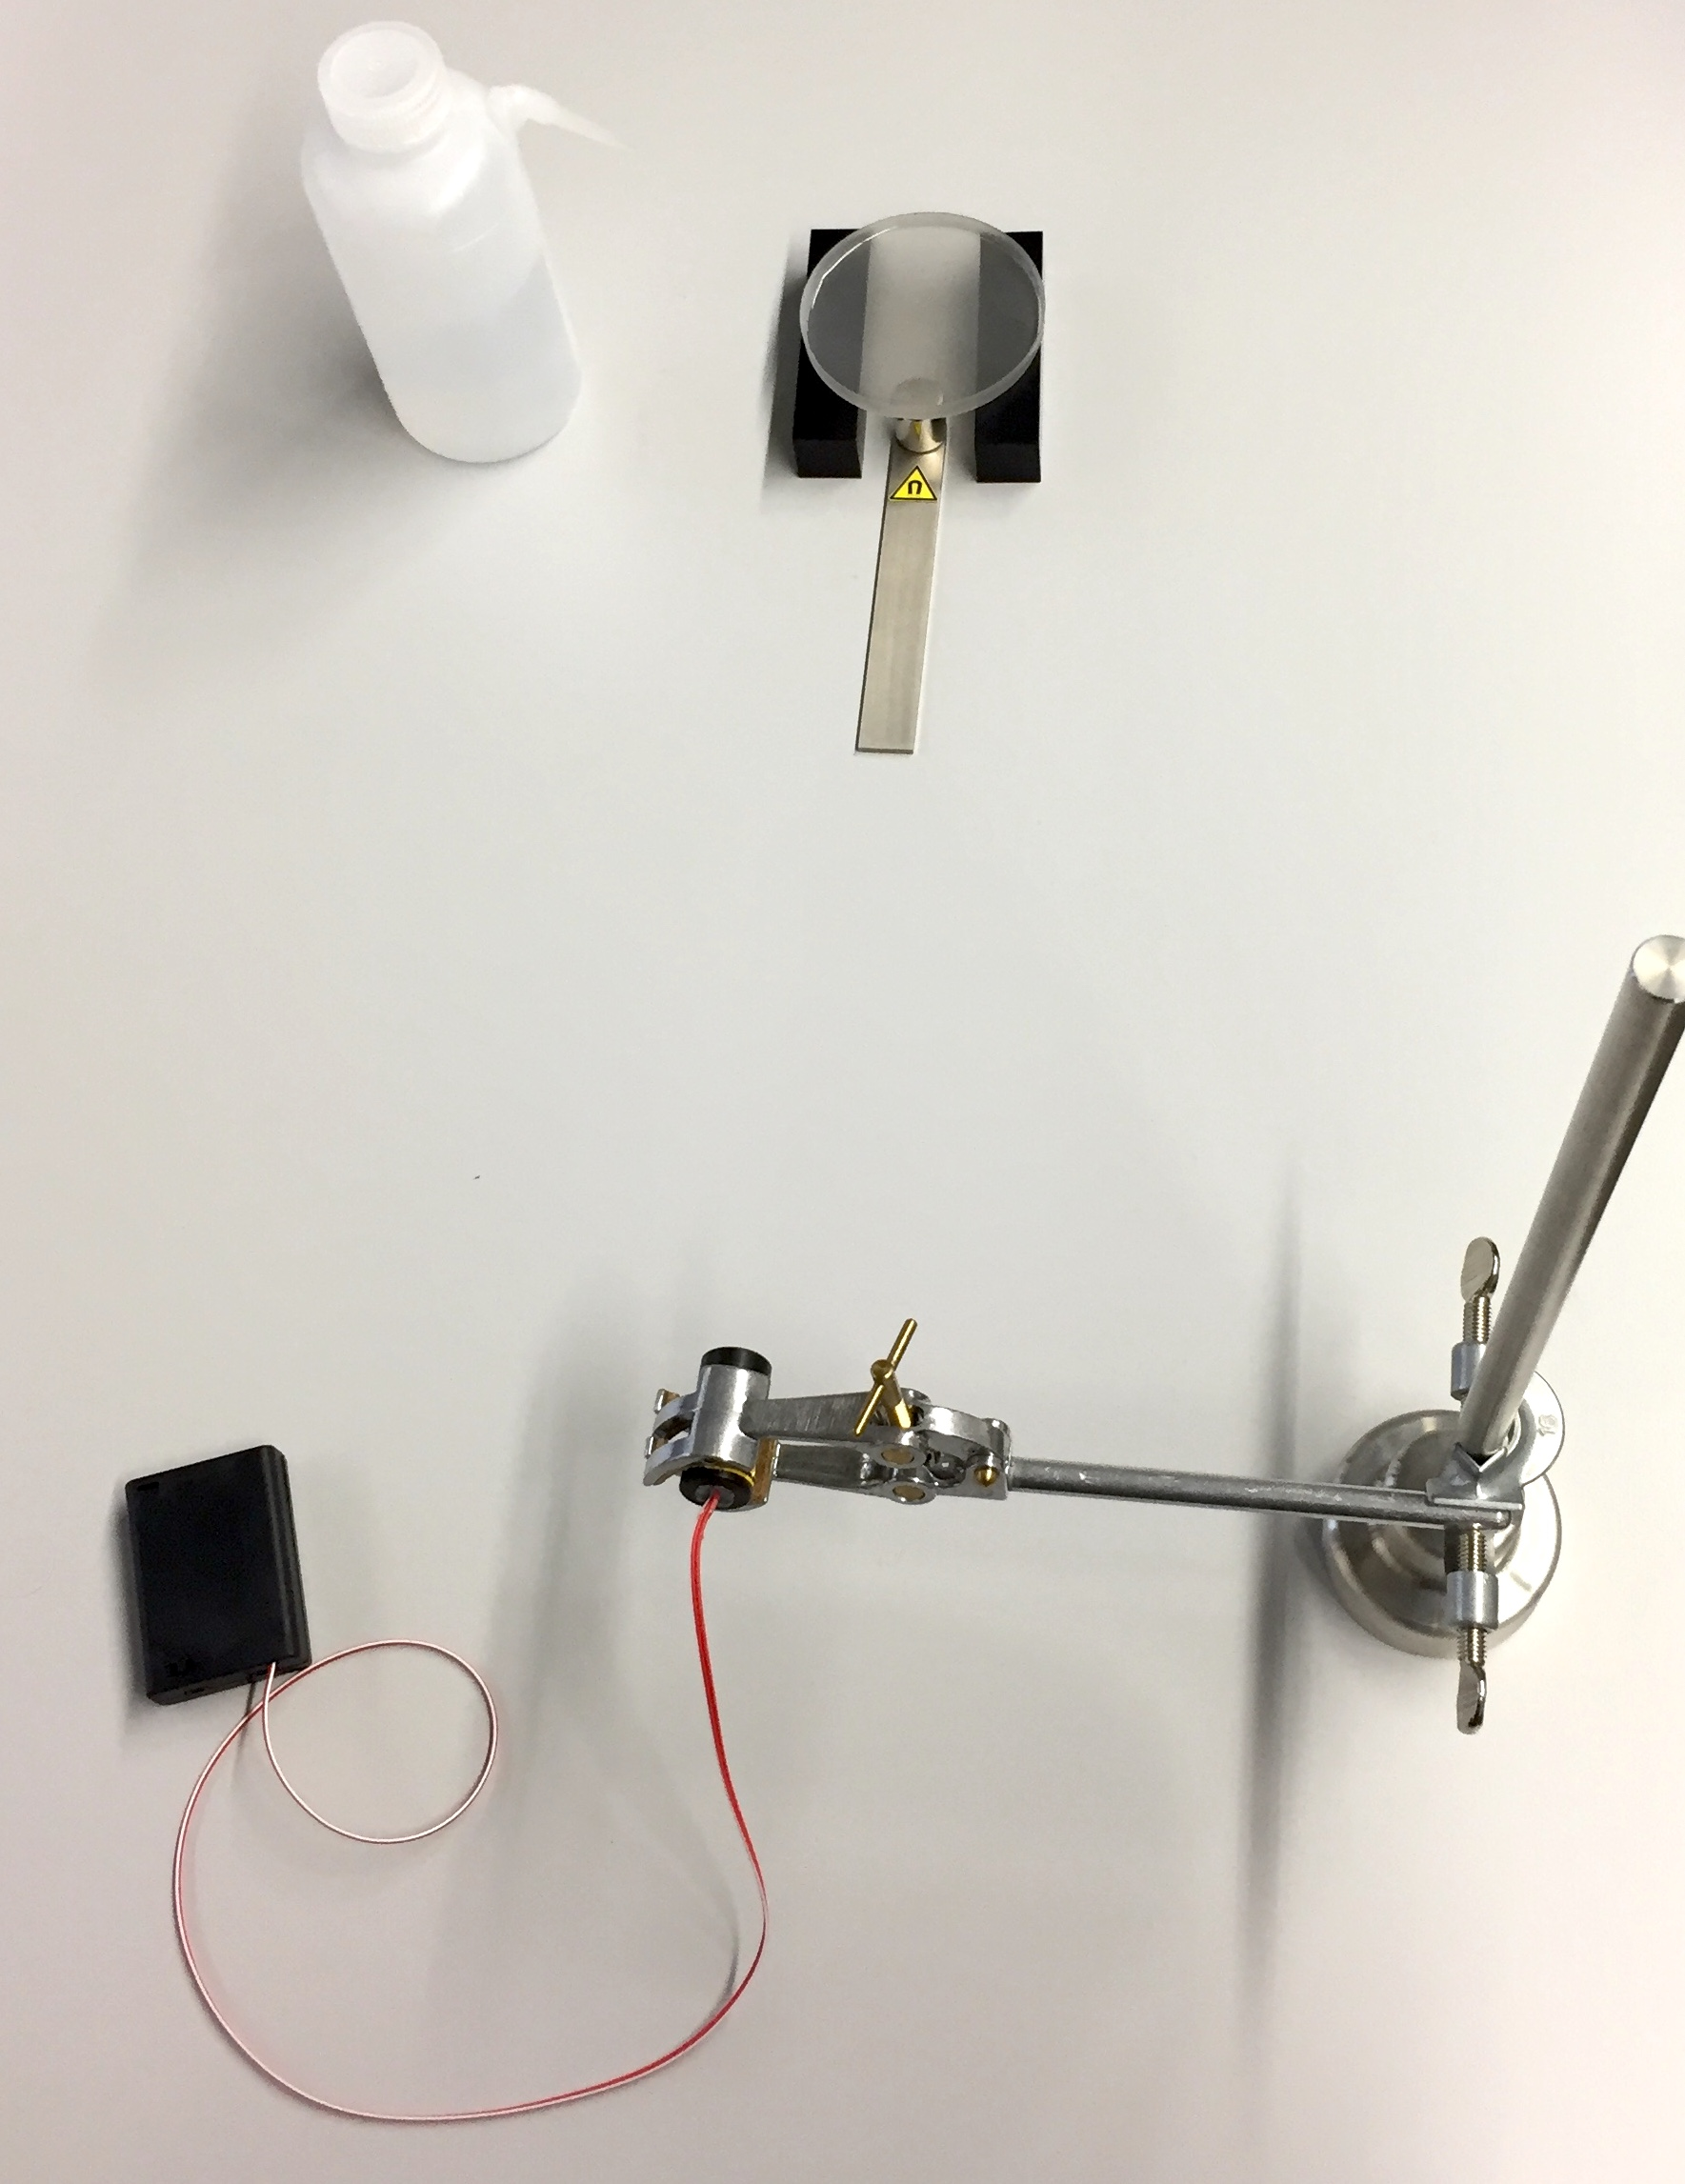
\includegraphics[width=0.5\textwidth]{res/Wasser.jpg}
	\caption{Zusehen ist hier der Versuchsaufbau mit dem der Einfluss eines Magnetfeldes auf Wasser untersucht wurde\protect\footnotemark.}
	\label{fig:Aufbau}
\end{figure}
\footnotetext{Entnommen am 20.11.17  aus dem Learnweb Kurs "Experimentelle Übungen I 17-18"}